%
% A header that lets you compile a chapter by itself, or inside a larger document.
% Adapted from http://stackoverflow.com/questions/3655454/conditional-import-in-latex
%
%
%Use \inbpdocument and \outbpdocument in your individual files, in place of \begin{document} and \end{document}. In your main file, put in a \def \ismaindoc {} before including or importing anything.
%
% David Duvenaud
% June 2011
% 
% ======================================
%
%


\ifx\ismaindoc\undefined
	\newcommand{\inbpdocument}{
		\def \ismaindoc {}
		% Use this header if we are compiling by ourselves.
		\documentclass[a4paper,11pt,authoryear,index]{common/PhDThesisPSnPDF}
		
%\usepackage{draftwatermark}
%\SetWatermarkLightness{0.95}

% ******************************************************************************
% ****************************** Custom Margin *********************************

% Add `custommargin' in the document class options to use this section
% Set {innerside margin / outerside margin / topmargin / bottom margin}  and
% other page dimensions

\ifsetMargin
\else
    \RequirePackage[left=37mm,right=30mm,top=35mm,bottom=30mm]{geometry}
    \setFancyHdr % To apply fancy header after geometry package is loaded
\fi


%\chead{Unfinished draft}
%\cfoot{\texttt{Unfinished draft - compiled on \today{} at \currenttime}}

% *****************************************************************************
% ******************* Fonts (like different typewriter fonts etc.)*************

% Add `customfont' in the document class option to use this section

\ifsetFont
\else
    % Set your custom font here and use `customfont' in options. Leave empty to
    % load computer modern font (default LaTeX font).  

    \RequirePackage{libertine} 
\fi

% *****************************************************************************
% *************************** Bibliography  and References ********************

%\usepackage{cleveref} %Referencing without need to explicitly state fig /table

% Add `custombib' in the document class option to use this section
\ifsetBib % True, Bibliography option is chosen in class options
\else % If custom bibliography style chosen then load bibstyle here

   \RequirePackage[square, sort, numbers, authoryear]{natbib} % CustomBib

% If you would like to use biblatex for your reference management, as opposed to the default `natbibpackage` pass the option `custombib` in the document class. Comment out the previous line to make sure you don't load the natbib package. Uncomment the following lines and specify the location of references.bib file

% \RequirePackage[backend=biber, style=numeric-comp, citestyle=numeric, sorting=nty, natbib=true]{biblatex}
% \bibliography{References/references} %Location of references.bib only for biblatex

\fi


% changes the default name `Bibliography` -> `References'
\renewcommand{\bibname}{References}


% *****************************************************************************
% *************** Changing the Visual Style of Chapter Headings ***************
% Uncomment the section below. Requires titlesec package.

%\RequirePackage{titlesec}
%\newcommand{\PreContentTitleFormat}{\titleformat{\chapter}[display]{\scshape\Large}
%{\Large\filleft{\chaptertitlename} \Huge\thechapter}
%{1ex}{}
%[\vspace{1ex}\titlerule]}
%\newcommand{\ContentTitleFormat}{\titleformat{\chapter}[display]{\scshape\huge}
%{\Large\filleft{\chaptertitlename} \Huge\thechapter}{1ex}
%{\titlerule\vspace{1ex}\filright}
%[\vspace{1ex}\titlerule]}
%\newcommand{\PostContentTitleFormat}{\PreContentTitleFormat}
%\PreContentTitleFormat


% *****************************************************************************
% **************************** Custom Packages ********************************
% *****************************************************************************


% ************************* Algorithms and Pseudocode **************************

%\usepackage{algpseudocode} 


% ********************Captions and Hyperreferencing / URL **********************

% Captions: This makes captions of figures use a boldfaced small font. 
%\RequirePackage[small,bf]{caption}

\RequirePackage[labelsep=space,tableposition=top]{caption} 
%\renewcommand{\figurename}{Figure} %to support older versions of captions.sty
\captionsetup{belowskip=12pt,aboveskip=4pt}

% ************************ Formatting / Footnote *******************************

%\usepackage[perpage]{footmisc} %Range of footnote options 


% ****************************** Line Numbers **********************************

%\RequirePackage{lineno}
%\linenumbers

% ************************** Graphics and figures *****************************

%\usepackage{rotating}
%\usepackage{wrapfig}
%\usepackage{float}
\usepackage{subfig} %note: subfig must be included after the `caption` package. 


% ********************************* Table **************************************

%\usepackage{longtable}
%\usepackage{multicol}
%\usepackage{multirow}
%\usepackage{tabularx}


% ***************************** Math and SI Units ******************************

\usepackage{amsfonts}
\usepackage{amsmath}
\usepackage{amssymb}
%\usepackage{siunitx} % use this package module for SI units


% ******************************************************************************
% ************************* User Defined Commands ******************************
% ******************************************************************************

% *********** To change the name of Table of Contents / LOF and LOT ************

%\renewcommand{\contentsname}{My Table of Contents}
%\renewcommand{\listfigurename}{List of figures}
%\renewcommand{\listtablename}{List of tables}


% ********************** TOC depth and numbering depth *************************

\setcounter{secnumdepth}{2}
\setcounter{tocdepth}{2}

% ******************************* Nomenclature *********************************

% To change the name of the Nomenclature section, uncomment the following line

%\renewcommand{\nomname}{Symbols}


% ********************************* Appendix ***********************************

% The default value of both \appendixtocname and \appendixpagename is `Appendices'. These names can all be changed via: 

%\renewcommand{\appendixtocname}{List of appendices}
%\renewcommand{\appendixname}{Appndx}

		% All my custom preamble stuff.  Shouldn't overlap with anything in official-preamble


% Paths to figure and table directories.
\newcommand{\symmetryfigsdir}{figures/symmetries}
\newcommand{\topologyfiguresdir}{figures/topology}
\newcommand{\infinitefiguresdir}{figures/infinite}
\newcommand{\grammarfiguresdir}{figures/grammar}
\newcommand{\introfigsdir}{figures/intro}
\newcommand{\gplvmfiguresdir}{figures/gplvm}
\newcommand{\warpedfiguresdir}{figures/warped-mixtures}
\newcommand{\deeplimitsfiguresdir}{figures/deep-limits}
\newcommand{\quadraturefigsdir}{figures/quadrature}
\newcommand{\additivefigsdir}{figures/additive}
\newcommand{\decompfigsdir}{figures/decomp}
\newcommand{\examplefigsdir}{figures/worked-example}


\usepackage{bm}  % for warped mixtures - is this necessary?
\usepackage{booktabs}
\usepackage{tabularx}
\usepackage{multirow}
\usepackage{datetime}
\renewcommand{\tabularxcolumn}[1]{>{\arraybackslash}m{#1}}
\usepackage{relsize}
\usepackage{graphicx}
\usepackage{amsmath,amssymb,textcomp}
\usepackage{nicefrac}
\usepackage{amsthm}
\usepackage{tikz}
\usetikzlibrary{arrows}
\usetikzlibrary{calc}
\usepackage{nth}
\usepackage{rotating}
\usepackage{array}
\usepackage{fp}
\usepackage[hyperpageref]{backref}
\def\foo{\hspace{\fill}\mbox{}\linebreak[0]\hspace*{\fill}}
\renewcommand*{\backref}[1]{}
\renewcommand*{\backrefalt}[4]{%
\ifcase #1 %
%
\or
\foo(page #2)%
\else
\foo(pages #2)%
\fi
}

\usepackage{cleveref}
\crefname{equation}{equation}{equations}


%% For submission, make all render blank.
%%%%%%%%%%%%%%%%%%%%%%%%%%%%%%%%%%%%%%%%%%%%%%%%%%%%%%%%%%
%%%% EDITING HELPER FUNCTIONS  %%%%%%%%%%%%%%%%%%%%%%%%%%%
%%%%%%%%%%%%%%%%%%%%%%%%%%%%%%%%%%%%%%%%%%%%%%%%%%%%%%%%%%

%% NA: needs attention (rough writing whose correctness needs to be verified)
%% TBD: instructions for how to fix a gap ("Describe the propagation by ...")
%% PROBLEM: bug or missing crucial bit 

%% use \fXXX versions of these macros to put additional explanation into a footnote.  
%% The idea is that we don't want to interrupt the flow of the paper or make it 
%% impossible to read because there are a bunch of comments.

%% NA's (and TBDs, those less crucially) should be written so 
%% that they flow with the text.

\definecolor{WowColor}{rgb}{.75,0,.75}
\definecolor{SubtleColor}{rgb}{0,0,.50}

% inline
\newcommand{\NA}[1]{\textcolor{SubtleColor}{ {\tiny \bf ($\star$)} #1}}
\newcommand{\LATER}[1]{\textcolor{SubtleColor}{ {\tiny \bf ($\dagger$)} #1}}
\newcommand{\TBD}[1]{\textcolor{SubtleColor}{ {\tiny \bf (!)} #1}}
\newcommand{\PROBLEM}[1]{\textcolor{WowColor}{ {\bf (!!)} {\bf #1}}}

% as margin notes

\newcounter{margincounter}
\newcommand{\displaycounter}{{\arabic{margincounter}}}
\newcommand{\incdisplaycounter}{{\stepcounter{margincounter}\arabic{margincounter}}}

\newcommand{\fTBD}[1]{\textcolor{SubtleColor}{$\,^{(\incdisplaycounter)}$}\marginpar{\tiny\textcolor{SubtleColor}{ {\tiny $(\displaycounter)$} #1}}}

\newcommand{\fPROBLEM}[1]{\textcolor{WowColor}{$\,^{((\incdisplaycounter))}$}\marginpar{\tiny\textcolor{WowColor}{ {\bf $\mathbf{((\displaycounter))}$} {\bf #1}}}}

\newcommand{\fLATER}[1]{\textcolor{SubtleColor}{$\,^{(\incdisplaycounter\dagger)}$}\marginpar{\tiny\textcolor{SubtleColor}{ {\tiny $(\displaycounter\dagger)$} #1}}}

%\renewcommand{\LATER}[1]{}
%\renewcommand{\fLATER}[1]{}
%\renewcommand{\TBD}[1]{}
%\renewcommand{\fTBD}[1]{}
%\renewcommand{\PROBLEM}[1]{}
%\renewcommand{\fPROBLEM}[1]{}
%\renewcommand{\NA}[1]{}


% HUMBLE WORDS: shown slightly smaller when in normal text
% Thanks to Christian Steinruecken!

% HUMBLE WORDS: shown slightly smaller when in normal text
%
\makeatletter%
%\def\@humbleformat#1{{\fontsize{}{1em}\selectfont #1}}
%\def\@humbleformat#1{\textsmaller{#1}}%
\newlength{\nonHumbleHeight}
\def\@humbleformat#1{{\settoheight{\nonHumbleHeight}{#1}\resizebox{!}{0.94\nonHumbleHeight}{#1}}}%
\def\@idxhumbleformat#1{{\relscale{0.95}{#1}}}%
%\def\@humbleformat#1{{#1}}%
\def\declareHumble#1#2{%
  \expandafter\def\csname #1\endcsname{\@humbleformat{#2}}%
  \expandafter\def\csname s#1\endcsname{{#2}}%
  \expandafter\def\csname idx#1\endcsname{{\@idxhumbleformat{#2}}}%
}%
\def\humble#1{\@humbleformat{#1}}%
\def\idxhumble#1{\@idxhumbleformat{#1}}%
\makeatother%

% Convenient indexing for humble abbreviations
\def\humbleindex#1#2{\index{#1@\idxhumble{#1}}}



% TODO: Clean up duplicates
\declareHumble{ANOVA}{ANOVA}
\declareHumble{ARD}{ARD}
\declareHumble{BIC}{BIC}
\declareHumble{BMC}{BMC}
\declareHumble{bq}{BQ}
\declareHumble{CRP}{CRP}
\declareHumble{dirpro}{DP}
\declareHumble{HDMR}{HDMR}
\declareHumble{GAM}{GAM}
\declareHumble{GEM}{GEM}
\declareHumble{GMM}{GMM}
\declareHumble{gplvm}{GP-LVM}
\declareHumble{gpml}{GPML}
\declareHumble{GPML}{GPML}
\declareHumble{gprn}{GPRN}
\declareHumble{gpt}{GP}
\declareHumble{gp}{GP}
\declareHumble{HKL}{HKL}
\declareHumble{HMC}{HMC}
\declareHumble{ibp}{IBP}
\declareHumble{iGMM}{iGMM}
\declareHumble{iwmm}{iWMM}
\declareHumble{kCP}{CP}
\declareHumble{kCW}{CW}
\declareHumble{kC}{C}
\declareHumble{KDE}{KDE}
\declareHumble{kLin}{Lin}
\declareHumble{KPCA}{KPCA}
\declareHumble{kPer}{Per}
\declareHumble{kRQ}{RQ}
\declareHumble{kSE}{SE}
\declareHumble{kWN}{WN}
\declareHumble{Lin}{Lin}
\declareHumble{LBFGS}{L-BFGS}
\declareHumble{mcmc}{MCMC}
\declareHumble{MKL}{MKL}
\declareHumble{MLP}{MLP}
\declareHumble{MSE}{MSE}
\declareHumble{Per}{Per}
\declareHumble{RMSE}{RMSE}
\declareHumble{RQ}{RQ}
\declareHumble{SBQ}{SBQ}
\declareHumble{seard}{SE-ARD}
\declareHumble{sefull}{SE-\textnormal{full}}
\declareHumble{SEGP}{SE-GP}
\declareHumble{SE}{SE}
\declareHumble{SNR}{SNR}
\declareHumble{SSANOVA}{SS-ANOVA}
\declareHumble{SVM}{SVM}

\newcommand{\kSig}{\boldsymbol\sigma}

\def\subexpr{{\cal S}}
\def\baseker{{\cal B}}
\def\numWinners{k}

\def\ie{i.e.\ }
\def\eg{e.g.\ }
\def\etc{etc.\ }
\let\oldemptyset\emptyset
\let\emptyset 0




% Unify notation between neural-net land and GP-land.
\newcommand{\hphi}{h}
\newcommand{\hPhi}{\vh}
\newcommand{\walpha}{w}
\newcommand{\wboldalpha}{\bw}
\newcommand{\wcapalpha}{\vW}
\newcommand{\lengthscale}{w}

\newcommand{\layerindex}{\ell}



\newcommand{\gpdrawbox}[1]{
\setlength\fboxsep{0pt}
\hspace{-0.15in} 
\fbox{
\includegraphics[width=0.464\columnwidth]{\deeplimitsfiguresdir/deep_draws/deep_gp_sample_layer_#1}
}}



\newcommand{\procedurename}{ABCD}
\newcommand{\genText}[1]{{\sf #1}}



\newcommand{\asdf}{$^{\textnormal{th}}$}

\newcommand{\binarysum}{\sum_{\bf{x} \in \{0,1\}^D}}
\newcommand{\expect}{\mathbb{E}}
\newcommand{\expectargs}[2]{\mathbb{E}_{#1} \left[ {#2} \right]}
\newcommand{\var}{\mathbb{V}}
\newcommand{\varianceargs}[2]{\mathbb{V}_{#1} \left[ {#2} \right]}
\newcommand{\cov}{\operatorname{cov}}
\newcommand{\Cov}{\operatorname{Cov}}
\newcommand{\covargs}[2]{\cov \left[ {#1}, {#2} \right]}
\newcommand{\variance}{\mathbb{V}}
\newcommand{\vecop}[1]{\operatorname{vec} \left( {#1} \right)}

\newcommand{\covarianceargs}[2]{\Cov_{#1} \left[ {#2} \right]}
\newcommand{\colvec}[2]{\left[ \begin{array}{c} {#1} \\ {#2} \end{array} \right]}
\newcommand{\tbtmat}[4]{\left[ \begin{array}{cc} {#1} & {#2} \\ {#3} & {#4} \end{array} \right]}

%\newcommand{\covskinny}[2]{\var\!\left(#1\middle\vert#2\right)} 

\newcommand{\acro}[1]{{\humble{#1}}}
%\newcommand{\vect}[1]{\boldsymbol{#1}}
\newcommand{\vect}[1]{{\bf{#1}}}
\newcommand{\mat}[1]{\mathbf{#1}}
\newcommand{\pderiv}[2]{\frac{\partial #1}{\partial #2}}
\newcommand{\npderiv}[2]{\nicefrac{\partial #1}{\partial #2}}

\newcommand{\pha}{^{\phantom{:}}}

\newcommand{\argmin}{\operatornamewithlimits{argmin}}
\newcommand{\argmax}{\operatornamewithlimits{argmax}}

% The following designed for probabilities with long arguments

\newcommand{\Prob}[2]{P\!\left(\,#1\;\middle\vert\;#2\,\right)}
\newcommand{\ProbF}[3]{P\!\left(\,#1\!=\!#2\;\middle\vert\;#3\,\right)}
\newcommand{\p}[2]{p\!\left(#1\middle\vert#2\right)}
\newcommand{\po}[1]{p\!\left(#1\right)}
\newcommand{\pF}[3]{p\!\left(\,#1\!=\!#2\;\middle\vert\;#3\,\right)} 
\newcommand{\mean}[2]{{m}\!\left(#1\middle\vert#2\right)}



\newcommand{\valpha}{\boldsymbol{\alpha}}
\newcommand{\va}{\vect{a}}
\newcommand{\vA}{\vect{A}}
\newcommand{\vB}{\mat{B}}
\newcommand{\vb}{\vect{b}}
\newcommand{\vC}{\mat{C}}
\newcommand{\vc}{\vect{c}}
\newcommand{\vecf}{\boldsymbol{f}}
\newcommand{\vell}{\vect{\ell}}
\newcommand{\vepsilon}{\boldsymbol{\epsilon}}
\newcommand{\veps}{\boldsymbol{\epsilon}}
\newcommand{\ve}{\boldsymbol{\epsilon}}
\newcommand{\vf}{\vecf}
\newcommand{\vg}{\vect{g}}
\newcommand{\vh}{\vect{h}}
\newcommand{\vI}{\mat{I}}
\newcommand{\vK}{\mat{K}}
\newcommand{\vk}{\vect{k}}
\newcommand{\vL}{\mat{L}}
\newcommand{\vl}{\vect{l}}
\newcommand{\vmu}{\boldsymbol{\mu}}
\newcommand{\vone}{\vect{1}}
\newcommand{\vphi}{\boldsymbol{\phi}}
\newcommand{\vpi}{\boldsymbol{\pi}}
\newcommand{\vq}{\vect{q}}
\newcommand{\vR}{\mat{R}}
\newcommand{\vr}{\vect{r}}
\newcommand{\vsigma}{\boldsymbol{\sigma}}
\newcommand{\vSigma}{\mat{\Sigma}}
\newcommand{\vS}{\mat{S}}
\newcommand{\vs}{\vect{s}}
\newcommand{\vtheta}{\boldsymbol{\theta}}
\newcommand{\vu}{\vect{u}}
\newcommand{\vV}{\mat{V}}
\newcommand{\vW}{\mat{W}}
\newcommand{\vw}{\vect{w}}
\newcommand{\vX}{\mat{X}}
\newcommand{\vx}{\vect{x}}
\newcommand{\vY}{\mat{Y}}
\newcommand{\vy}{\vect{y}}
\newcommand{\vzero}{\vect{0}}
\newcommand{\vZ}{\mat{Z}}
\newcommand{\vz}{\vect{z}}


\newcommand{\netweights}{\alpha}
\newcommand{\vnetweights}{\valpha}

\newcommand{\He}{\mathcal{H}}
\newcommand{\normx}[2]{\left\|#1\right\|_{#2}}
\newcommand{\Hnorm}[1]{\normx{#1}{\He}}
\newcommand{\mmd}{{\rm MMD}}


\newcommand{\mf}{\bar{\vf}}

%\newcommand{\mf}{\mu} %{\bar{\ell}}
\newcommand{\lf}{f} % Likelihood function
\newcommand{\st}{_\star}

% from simpler log-bq writeup
\newcommand{\lftwo}{{\log \ell}}
\newcommand{\mftwo}{{\bar \ell}}
\newcommand{\loggp}{{\log\acro{GP}}}%| \bX, \vy )}}
\newcommand{\loggpdist}{{\acro{GP}(\lftwo)}}%| \vX, \vy )}}


\newcommand{\inv}{^{{\mathsmaller{-1}}}}
\newcommand{\tohalf}{^{{\mathsmaller{\nicefrac{1}{2}}}}}

\newcommand{\Normal}{\mathcal{N}}
\newcommand{\N}[3]{\mathcal{N}\!\left(#1 \middle| #2,#3\right)}
\newcommand{\Nt}[2]{\mathcal{N}\!\left(#1,#2\right)}
\newcommand{\NT}[2]{\mathcal{N}\!\left(#1,#2\right)}
\newcommand{\GPdist}[3]{\mathcal{GP}\!\left(#1 \, \middle| \, #2, #3 \right)}
\newcommand{\bN}[3]{\mathcal{N}\big(#1 \middle| #2,#3\big)}
\newcommand{\boldN}[3]{\text{\textbf{\mathcal{N}}}\big(#1;#2,#3\big)}
\newcommand{\ones}[1]{\mat{1}_{#1}}
\newcommand{\eye}[1]{\mat{E}_{#1}}
\newcommand{\tra}{^{\mathsf{T}}}
%\newcommand{\tra}{^{\top}}
%\mathsf{T}
\newcommand{\trace}{\operatorname{tr}}
\newcommand{\shift}{\operatorname{shift}}
\renewcommand{\mod}{\operatorname{mod}}
\newcommand{\deq}{:=}
\newcommand{\oneofk}{\operatorname{one-of-k}}
%\newcommand{\degree}{^\circ}

\newcommand{\GPt}[2]{\mathcal{GP}\!\left(#1,#2\right)}
%\newcommand{\GPt}[2]{\gp\!\left(#1,#2\right)}

\DeclareMathOperator{\tr}{tr}
\DeclareMathOperator{\chol}{chol}
\DeclareMathOperator{\diag}{diag}

\newenvironment{narrow}[2]{%
  \begin{list}{}{%
  \setlength{\topsep}{0pt}%
  \setlength{\leftmargin}{#1}%
  \setlength{\rightmargin}{#2}%
  \setlength{\listparindent}{\parindent}%
  \setlength{\itemindent}{\parindent}%
  \setlength{\parsep}{\parskip}}%
\item[]}{\end{list}}



\newcommand{\dist}{\ \sim\ }
\def\given{\,|\,}

% Table stuff
\newcolumntype{C}[1]{>{\centering\let\newline\\\arraybackslash\hspace{0pt}}m{#1}}
\newcolumntype{L}[1]{>{\raggedright\let\newline\\\arraybackslash\hspace{0pt}}m{#1}}
\newcolumntype{R}[1]{>{\raggedleft\let\newline\\\arraybackslash\hspace{0pt}}m{#1}}


\def\ie{i.e.\ }
\def\eg{e.g.\ }
\def\iid{i.i.d.\ }
%\def\simiid{\sim_{\mbox{\tiny iid}}}
\def\simiid{\overset{\mbox{\tiny iid}}{\sim}}
\def\simind{\overset{\mbox{\tiny \textnormal{ind}}}{\sim}}
\def\eqdist{\stackrel{\mbox{\tiny d}}{=}}
%\newcommand{\distas}[1]{\mathbin{\overset{#1}{\kern \z@ \sim}}}
%TODO: fix this - it worked outside the thesis!
\newcommand{\distas}[1]{\mathbin{\overset{#1}{\sim}}}

\def\Reals{\mathbb{R}}

\def\Uniform{\mbox{\rm Uniform}}
\def\Bernoulli{\mbox{\rm Bernoulli}}
\def\GP{\mathcal{GP}}
\def\GPLVM{\mathcal{GP-LVM}}




% Kernel stuff

\def\iva{\vect{\inputVar}}
\def\ivaone{\inputVar}
\def\inputVar{x}
\def\InputVar{X}
\def\InputSpace{\mathcal{X}}
\def\outputVar{y}
\def\OutputSpace{\mathcal{Y}}
\def\function{f}
\def\kernel{k}
\def\KernelMatrix{K}
\def\SumKernel{\sum}
\def\ProductKernel{\prod}
\def\expression{e}
\def\feat{\vh}

\newcommand{\kerntimes}{ \! \times \!}
\newcommand{\kernplus}{ \, + \,}


% Proof stuff
\theoremstyle{plain}
\newtheorem{theorem}{Theorem}[section]
\newtheorem{lemma}[theorem]{Lemma}
\newtheorem{prop}[theorem]{Proposition}
\newtheorem{proposition}{Proposition}
\newtheorem*{cor}{Corollary}

% For infinite bq
\newcommand{\iv}{\theta}
\newcommand{\viv}{\vtheta}

% For intro chapter
\newcommand{\funcval}{\vf(\vX)}
\newcommand{\testpoint}{{\vx^\star}}

\newcommand{\underwrite}[2]{{\underbrace{#1}_{\textnormal{#2}}}}



% For kernel figures
\newcommand{\fhbig}{2cm}%
\newcommand{\fwbig}{3cm}%
\newcommand{\kernpic}[1]{\includegraphics[height=\fhbig,width=\fwbig]{\grammarfiguresdir/structure_examples/#1}}%
\newcommand{\kernpicr}[1]{\rotatebox{90}{\includegraphics[height=\fwbig,width=\fhbig]{\grammarfiguresdir/structure_examples/#1}}}%
\newcommand{\addkernpic}[1]{{\includegraphics[height=\fhbig,width=\fwbig]{\grammarfiguresdir/additive_multi_d/#1}}}%
\newcommand{\largeplus}{\tabbox{{\Large+}}}%
\newcommand{\largeeq}{\tabbox{{\Large=}}}%
\newcommand{\largetimes}{\tabbox{{\Large$\times$}}}%
\newcommand{\fixedx}{$x$ (with $x' = 1$)}%


		% ************************ Thesis Information & Meta-data **********************

%% The title of the thesis
%\title{Structured Gaussian Process Models} 
%\title{Automatic Model Construction \\ through \\ Structured Gaussian Processes}
%\title{Automatic Model-Building \\ through \\ Structured Gaussian Processes}
%\title{Automatic Modeling \\ with \\ Structured Gaussian Processes}    
\title{Automatic Model Construction \\ with Gaussian Processes}
%\title{Automatic Model Construction}
%\title{Automating Statistical Model Construction}


%\texorpdfstring is used for PDF metadata. Usage:
%\texorpdfstring{LaTeX_Version}{PDF Version (non-latex)} eg.,
%\texorpdfstring{$sigma$}{sigma}

%% The full name of the author
\author{David Kristjanson Duvenaud}

%% Department (eg. Department of Engineering, Maths, Physics)
%\dept{Department of Engineering}

%% University and Crest
\university{University of Cambridge}
\crest{
\includegraphics[width=0.25\textwidth]{University_Crest}}

%% You can redefine the submission text:
% Default as per the University guidelines: This dissertation is submitted for
% the degree of Doctor of Philosophy
%\renewcommand{\submissiontext}{change the default text here if needed}

%% Full title of the Degree 
\degree{Doctor of Philosophy}
 
%% College affiliation (optional)
\college{Pembroke College}

%% Submission date
\degreedate{June 2014} 

%% Meta information
\subject{LaTeX} \keywords{{LaTeX} {PhD Thesis} {Engineering} {University of Cambridge}}



		\begin{document}
	}	
	\newcommand{\outbpdocument}[1]{

		% Fake chapters so references aren't broken
\label{ch:intro}                
\label{ch:kernels}
\label{ch:grammar}
\label{ch:description}
\label{ch:additive}
\label{ch:deeplimits}
\label{ch:discussion}
		%\bibliographystyle{common/CUEDthesis}
		\bibliographystyle{plainnat}
		\bibliography{references.bib}
		\end{document}
	}	
\else
	%If we're inside another document, no need to re-start the document.
	\ifx\inbpdocument\undefined
		\newcommand{\inbpdocument}{}
		\newcommand{\outbpdocument}[1]{}
	\fi
\fi

\inbpdocument


\chapter{Automatically Building Structured Covariance Functions}
\label{ch:grammar}

\begin{quotation}
``It would be very nice to have a formal apparatus that gives us some `optimal' way of recognizing unusual phenomena and inventing new classes of hypotheses that are most likely to contain the true one; but this remains an art for the creative human mind.''
%``It would be very nice to have a formal apparatus that gives us some `optimal' way of recognizing unusual phenomena and inventing new classes of hypotheses \dots but this remains an art for the creative human mind.''
% In trying to practice this art, the Bayesian has the advantage because his formal apparatus already developed gives him a clearer picture of what to expect, and therefore a sharper perception for recognizing the unexpected.

\defcitealias{Jaynes85highlyinformative}{E. T.  Jaynes, 1985}
\hspace*{\fill}\citetalias{Jaynes85highlyinformative}
\end{quotation}


In \cref{ch:kernels}, we saw that the choice of kernel determines the type of structure that can be learnt by a \gp{} model, and that a wide variety of models could be constructed through simply adding and multiplying a few base kernels together.
We didn't answer the question, however, of how to tell which kernel to use for a given problem.
Even for experts, choosing the kernel in nonparametric regression remains something of a black art.

In this chapter, we'll automate the process of building kernels for \gp{} models.
To do so, we need to define an open-ended space of kernels; we'll do this by simply adding and multiplying together simple kernels from a fixed set.
We can then simply search over this space to find a kernel which captures as much structure in the data as possible.

Searching over such a large, structured model class has two main benefits.
First, this procedure has very good predictive accuracy, since it tries out a large number of different regression models.
Second, this procedure can discover interpretable structure in datasets.
Because \gp{} posteriors can be decomposed (as in \cref{sec:concrete}), we can also examine the resulting structures visually.
In \cref{ch:description}, we'll even show how to automatically generate english-language descriptions of the resulting models.

%Section \ref{sec:Structure} outlines some commonly used kernel families as well as ways in which they can be composed. 
%Our grammar over kernels and our proposed structure discovery algorithm are described in Section \ref{sec:Search}. 
%Section \ref{sec:related_work} situates our work in the context of other nonparametric regression, kernel learning, and structure discovery methods.
%We evaluate our methods on synthetic datasets, time series analysis, and high-dimensional prediction problems in Sections \ref{sec:synthetic} through \ref{sec:quantitative}, respectively.

%What are the ingredients required for an artificial intelligence system to be able to perform statistical modeling automatically? 
%In this paper we conjecture that the following ingredients may be useful for building an AI system for statistics, and we develop a working system which incorporates them:
%\begin{itemize}
%\item {\bf An open-ended language of models} expressive enough to capture many of the modeling assumptions and model composition techniques  applied by human statisticians to capture real-world phenomena
%\item {\bf A search procedure} to efficiently explore the space of models spanned by the language
%\item {\bf A principled method for evaluating models} in terms of their complexity and their degree of fit to the data
%\item {\bf A procedure for automatically generating reports} which can explain and visualize different factors underlying the data, make the chosen modeling assumptions explicit, and quantify how each component improves the predictive power of the model 
%\end{itemize}


\section{Ingredients of an Automatic Statistician}
\label{sec:ingredients}
\citet{gelman2013philblogpost} asks ``How can an artificial intelligence do statistics? ... It needs not just an inference engine, but also a way to construct new models and a way to check models. Currently, those steps are performed by humans, but the AI would have to do it itself.''

In this section, we discuss in more detail the elements we believe are required to build an artificial intelligence that can do statistics.

\paragraph{1. An open-ended language of models}
Many statistical procedures consider all models in a class of fixed size - for example, graphical model construction algorithms\fTBD{Cite} search over connectivity graphs for a given set of nodes.
While these methods can be powerful, human statisticians are capable of deriving novel model classes when required.
An automatic search through an open-ended class of models can achieve some of this flexibility, growing the complexity of the model to fit the task at hand, and possibly combining existing structures in novel ways.

\paragraph{2. A Search through model space}
An open-ended space of models cannot be searched exhaustively.
Just as human researchers iteratively refine their models, search procedures can propose new search directions based on the results of previous model fits.
Because any search in an open-ended space must start with relatively simple models before moving on to more complex ones, any model search in an open-ended space will likely resemble a model-building procedure.% based 

\paragraph{3. A Model comparison procedure}
An automatic statistician should be able to question the models it has constructed, and formal procedures from model checking provide a way for it to do this.
\citet{gelman2012philosophy} review the literature on model checking.
In this work, we use approximate marginal likelihood to compare models, penalizing complexity using the Bayesian Information Criterion as a heuristic.

\paragraph{4. A model description procedure}
Part of the value of statistical models comes from enabling humans to understand a dataset or a phenomenon.
Furthermore, a clear description of the statistical structure found in a dataset helps a user to notice when the dataset has errors, the wrong question was asked, the model-building procedure failed to capture known structure, a relevant piece of data or constraint is missing, or when a novel statistical structure has been found.
%In this chapter, we'll show how the additive decomposition of \gp{} posteriors allows a visual description of composite \gp{} models.
%In \cref{ch:description}, we'll further show how to automatically generate english-language descriptions of the resulting models.





In this chapter, we introduce a system containing all the above ingredients.
We call this system the Automatic Bayesian Covariance Discovery (\procedurename{}) system.
The next four sections of this chapter describe the mechanisms we use to produce these four ingredients, for this particular example of an artificial intelligence which does statistics.



\section{A Language of Regression Models}
\label{sec:improvements}

As shown in Chapter~\ref{ch:kernels}, we can construct a wide variety of kernel structures compositionally by adding and multiplying a small number of base kernels.
We can therefore define a language of regression models by specifying a language of kernels.

The elements of this language are a set of base kernels capturing different function properties, and a set of
composition rules which combine kernels to yield other valid kernels.
In this chapter, we'll use such base kernels as white noise ($\kWN$), constant ($\kC$), linear ($\kLin$), squared-exponential ($\kSE$), rational-quadratic ($\kRQ$), sigmoidal ($\kSig$) and periodic ($\kPer$).
%, which on their own encode for uncorrelated noise, constant functions, linear functions, smooth functions and periodic functions respectively.

%
\begin{table}[h]%
\centering
\begin{tabular}{cccc}
Kernel name: & Rational quadratic (\kRQ) & Cosine ($\cos$) & White noise (\kLin) \\[10pt]
$k(x, x') =$ & $\exp\left(-\frac{(\inputVar - \inputVar')^2}{2\ell^2}\right)$ &
$\cos\left(\frac{2 \pi (x - x')}{p}\right)$ &
$\delta(\inputVar - \inputVar')$ \\[14pt]
\raisebox{1cm}{Plot of kernel:} & \kernpic{rq_kernel} & \kernpic{cos_kernel} & \kernpic{wn_kernel}\\
& $x -x'$ & $x -x'$ & \fixedx \\
%& & & \\
 & \large $\downarrow$ & \large $\downarrow$ & \large $\downarrow$  \\
\raisebox{1cm}{Samples from prior:} & \kernpic{rq_kernel_draws_s4} & \kernpic{cos_kernel_draws_s1} & \kernpic{wn_kernel_draws_s1} \\
Type of structure: & multiscale variation & sine waves & uncorrelated noise\\[10pt]
\end{tabular}
\caption[Some other basic kernels]
{New base kernels introduced in this chapter, and the types of structure they encode.
More interesting kernels can be constructed by adding and multiplying base kernels together.
%Left and third columns: base kernels $k(\cdot,0)$.
%Second and fourth columns: draws from a \sgp{} with each repective kernel.
%The x-axis has the same range on all plots.
}
\label{fig:basic_kernels_two}
\end{table}
%
To specify an open-ended language of structured kernels, we'll consider the set of all kernels that can be built by adding and multiplying these base kernels together:
\begin{align}
%k_1 + k_2 =      & \,\, k_1(\vx, \vx') + k_2(\vx, \vx') \\
%k_1 \times k_2 = & \,\, k_1(\vx, \vx') \times k_2(\vx, \vx') \\
(k_1 + k_2)(\vx, \vx') =& \,\, k_1(\vx, \vx') + k_2(\vx, \vx')\\
(k_1 \times k_2)(\vx, \vx') =& \,\, k_1(\vx, \vx') \times k_2(\vx, \vx')
\end{align}


%We have found that incorporating changepoints into the language is essential for realistic models of time series (\eg figure~\ref{fig:periodic}).
%[todo: expand a little]


% Moved to kernels chapter.
%Changepoints can be defined through addition and multiplication with sigmoidal functions:
%\begin{align}
%\kCP(\kernel_1, \kernel_2) = \kernel_1 \times \boldsymbol\sigma + \kernel_2 \times \boldsymbol{\bar\sigma}
%\label{eq:cp}
%\end{align}
%where $\boldsymbol\sigma = \sigma(x)\sigma(x')$ and $\boldsymbol{\bar\sigma} = (1-\sigma(x))(1-\sigma(x'))$.
%Changewindows $\kCW(\cdot,\cdot)$ can be defined similarly by replacing $\sigma(x)$ with a product of two sigmoids.

%We also expanded and reparametrised the set of base kernels so that they were more amenable to automatic description and to extend the number of common regression models included in the language.

Table~\ref{table:motifs} lists common regression models that can be expressed by this language.
\begin{table}[ht]
\centering
\begin{tabular}{l|l|l}
Regression model & Kernel & Related work\\
\midrule
Linear regression & $\kC + \kLin + \kWN$ & \\
Kernel ridge regression & $\kSE + \kWN$ & \\
Linear Semiparametric & $\kLin + \kSE + \kWN$ & \citep[e.g.][]{ruppert2003semiparametric} \\
Multiple kernel learning & $\sum \kSE$ + \kWN & \citep[e.g.][]{bach2004multiple} \\
Trend, cyclical, irregular   & $\sum \kSE + \sum \kPer$ + \kWN & \citep{lind2006basic}\\
Fourier decomposition & $\kC + \sum \cos$ + \kWN & \\
Sparse spectrum \gp{}s & $\sum \cos$ + \kWN & \citep{lazaro2010sparse} \\
Spectral mixture & $\sum \SE \times \cos$ + \kWN & \citep{WilAda13} \\
Changepoints & \eg $\kCP(\kSE, \kSE) + \kWN$ & \citep[e.g.][]{garnett2010sequential} \\
Heteroscedasticity & \eg $\kSE + \kLin \times \kWN$ & \\
Additive + Flexible & $ \sum_d \kSE_d + \prod_d \kSE_d$ & \citep{plate1999accuracy} 
\end{tabular}
\caption[Common regression models expressible in the kernel language]
{Common regression models expressible by sums and products of base kernels.
$\cos$ is a special case of our reparametrised \skPer.
}
\label{table:motifs}
\end{table}





\section{A Model Search Procedure}

We explore the space of regression models using a greedy search.
At each stage, we choose the highest scoring kernel and expand it by applying all operators to all existing kernels, combining or replacing them with all possible base kernels:
%
\begin{center}
\begin{tabular}{rccc}
\textnormal{Replacement:}    & $\kernel$ & $\to$ & $\kernel'$\\
\textnormal{Addition:}       & $\kernel$ & $\to$ & $\kernel + \kernel'$\\
\textnormal{Multiplication:} & $\kernel$ &  $\to$ & $\kernel \times \kernel'$\\
\end{tabular}
\end{center}
%
We also include additional operators to incorporate changepoints.
A complete list is contained in Appendix [BLANK]. 

These operators can generate all possible algebraic expressions.
To see this, observe that if we restricted the $+$ and $\times$ rules to only apply to base kernels, we would obtain a context-free grammar which generates the set of algebraic expressions.

Our search operators are motivated by strategies that human researchers often use to construct kernels.
In particular,
\begin{itemize}
\item One can look for structure, such as periodicity, in the residuals of a model, and then extend the model to capture that structure.
This corresponds to adding a new kernel to the existing structure.
\item One can start with structure, such as linearity, which is assumed to hold globally, but find that it only holds locally.
This corresponds to multiplying a kernel structure by a local kernel, such as $\kSE$.
\item One can add features incrementally, analogous to algorithms like boosting, backfitting, or forward selection.
This corresponds to adding or multiplying with kernels on dimensions not yet included in the model.
\end{itemize}

%We stop the procedure at a fixed depth (typically 10), and return the best-scoring kernel over all depths.
%The fixed depth was enforcing solely for convencience - because the 

\begin{figure}[ht]
\centering
%\begin{tabular}{cc}
%\begin{minipage}[t][14cm][t]{0.65\columnwidth}
\newcommand{\treescale}{*1.5\columnwidth}
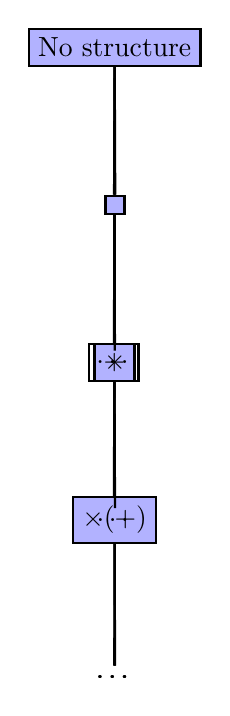
\begin{tikzpicture}
[sibling distance=0.15\treescale,-,thick, level distance=2cm]
%\footnotesize
\node[shape=rectangle,draw,thick,fill=blue!30] {No structure}
  child {node[shape=rectangle,draw,thick] {$\SE$}
  }
  child {node[shape=rectangle,draw,thick,fill=blue!30] {$\RQ$}
    [sibling distance=0.1\treescale]
    child {node[shape=rectangle,draw,thick] {$\SE$ + \RQ}}
    child {node {\ldots}}
    child {node[shape=rectangle,draw,thick,fill=blue!30] {$\Per + \RQ$}
      [sibling distance=0.15\treescale]
      child {node[shape=rectangle,draw,thick] {$\SE + \Per + \RQ$}}
      child {node {\ldots}}
      child {node[shape=rectangle,draw,thick,fill=blue!30] {$\SE \times (\Per + \RQ)$}
        [sibling distance=0.14\treescale]
        child {node {\ldots}}
        child {node {\ldots}}
        child {node {\ldots}}
      }
      child {node {\ldots}}
    }
    child {node {\ldots}}
    child {node[shape=rectangle,draw,thick] {$\Per \times \RQ$}}
  }
  child {node[shape=rectangle,draw,thick] {$\Lin$}
  }
  child {node[shape=rectangle,draw,thick] {$\Per$}
  };
\end{tikzpicture}
\caption[Search tree over kernels]{An example of a search tree over kernel expressions.
\Cref{fig:mauna_grow} shows the corresponding model increasing in sophistication as the kernel expression grows.
}
\label{fig:mauna_search_tree}
\end{figure}

\begin{figure}[ht!]
\centering
\newcommand{\wmg}{0.31\columnwidth}  % width maunu growth
\newcommand{\hmg}{3.2cm}  % height maunu growth
\newcommand{\maunadecomp}[1]{\hspace{-0.3cm}
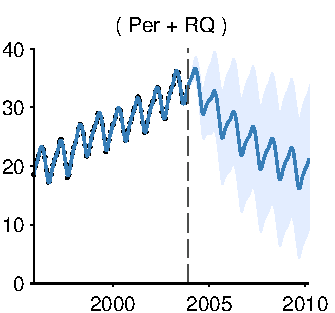
\includegraphics[width=\wmg,height=\hmg, clip,trim=0mm 0mm 0mm 7mm]{\grammarfiguresdir/decomposition/11-Feb-v4-03-mauna2003-s_max_level_#1/03-mauna2003-s_all_small}}
\begin{tabular}{ccc}
Level 1: & Level 2: & Level 3: \\
\RQ & $\Per + \RQ$ & $\SE \times (\Per + \RQ )$ \\[0.5em]
\maunadecomp{0} & \maunadecomp{1} & \maunadecomp{2} \\[0.5em]
\end{tabular}
\caption[Progression of models as the search depth increases]
{Posterior mean and variance for different depths of kernel search on the Mauna Loa dataset.
The dashed line marks the end of the dataset.
\emph{Left:} the function is only modeled as a locally smooth function, and the extrapolation is poor.
\emph{Middle:} a periodic component is added, and the extrapolation improves.
\emph{Right:} at depth 3, the kernel can capture most of the relevant structure, and is able to extrapolate reasonably.
}
\label{fig:mauna_grow}
\end{figure}

\Cref{fig:mauna_search_tree} shows an example search tree followed by our algorithm.
\Cref{fig:mauna_grow} shows how the resulting model changes as the search is followed.

\subsubsection{Hyperparameter initialization}

Unfortunately, optimizing the marginal likelihood over parameters is not a convex optimization problem, and the space can have many local optima.
For example, in data with periodic structure, integer multiples of the true period (harmonics) are often local optima. 
To alleviate this difficulty, we take advantage of our search procedure to provide reasonable initializations: all of the parameters which were part of the previous kernel are initialized to their previous values, while randomly initializing any newly introduced parameters.
In the newly proposed kernel, all parameters are then optimized using conjugate gradients.
This procedure is not guaranteed to find the global optimum, but it implements the commonly used heuristic of iteratively modeling residuals.







\section{A Model Comparison Procedure}

Choosing a kernel requires a method for comparing models.
We choose marginal likelihood as our criterion, since it balances the fit and complexity of a model \citep{rasmussen2001occam}.
Conditioned on kernel parameters, the marginal likelihood of a \gp{} can be computed analytically.
Given a parametric form of a kernel, we can also choose its parameters using marginal likelihood.
However, choosing kernel parameters by maximum likelihood raises the possibility of overfitting.
In addition, if we compare two classes of kernels by the maximum likelihood attainable over the kernel parameters, then all else being equal, the kernel class having more free parameters will always be chosen.

We could avoid overfitting by averaging the marginal likelihood over all free parameters, but this integral is hard to do in general.
Instead, we approximate this integral using the Bayesian information criterion (\BIC{}) \citep{schwarz1978estimating}:
%
\begin{equation}
\textrm{BIC}(M) = \log p(D \given M) - \frac{1}{2} |M| \log N
\end{equation}
%
where $p(D|M)$ is the marginal likelihood of the data (given by \cref{eq:gp_marg_lik}), $|M|$ is the number of kernel parameters, and $N$ is the number of data points.
\BIC{} simply penalizes the marginal likelihood in proportion to how many parameters the model has.
%BIC trades off model fit against model complexity and implements what is known as ``Bayesian Occam's Razor'' \citep{rasmussen2001occam,mackay2003information}.
Because BIC is a function of the number of parameters in a model, we adjusted for cases where two parameters were serving the role of one.  For example, when two kernels are multiplied, one of their output variance parameters becomes redundant.

Other more sophisticated approximations are possible, such as Laplace's approximation.
We chose to first try \BIC{} since it is the simplest thing that could possibly work, and it performed well in our experiments.




\section{A Model Description Procedure}

As discussed in \Cref{ch:kernels}, a \gp{} whose kernel is a sum of kernels can be viewed as a sum of functions drawn from different \gp{}s.
We can always express any kernel structure as a sum of products of kernels, by distributing all products of sums.
For example,
%
\begin{align}
\SE \kerntimes (\RQ \kernplus \Lin) = \SE \kerntimes  \RQ \kernplus \SE \kerntimes \Lin
\end{align}
%
This decomposition into additive components provides a method of visualizing the learned model, breaking down the different types of structure discovered in the data.

In \Cref{ch:description}, we'll extend this model visualization method to include automatically-generated english text explaining the meaning of each type of structure discovered.



\section{Structure Discovery in Time Series}
\label{sec:time_series}

To investigate our method's ability to discover structure, and to plausibly extrapolate, we ran the kernel search on several time-series.
In the following examples, the search was run to depth 10, using \kSE{}, \kRQ{}, \kLin{}, \kPer{} and \kWN{} as base kernels.

\label{sec:extrapolation}
\subsection{Mauna Loa atmospheric CO$\mathbf{_{2}}$}

Using our method, we analyzed records of carbon dioxide levels recorded at the Mauna Loa observatory.
Since this dataset was analyzed in detail by \citet{rasmussen38gaussian}, we can compare the kernel chosen by our method to a kernel constructed by human experts.


\begin{figure}[ht!]
\newcommand{\wmgd}{0.5\columnwidth}  % width mauna decomp
\newcommand{\hmgd}{3.51cm}  % height mauna decomp
\newcommand{\mdrd}{\grammarfiguresdir/decomposition/11-Feb-03-mauna2003-s}  % mauna decomp results dir
\newcommand{\mbm}{\hspace{-0.2cm}}  % move back
\newcommand{\maunadgfx}[1]{\mbm \includegraphics[width=\wmgd,height=\hmgd, clip, trim=0mm 0mm 0mm 6mm]{\mdrd/03-mauna2003-s_#1}}
\begin{tabular}{cc}
\multicolumn{2}{c}{
\begin{tabular}{c}
Complete Model: 
$\kLin \kerntimes \kSE + \kSE \kerntimes ( \kPer + \RQ ) + \kWN$ \\
\maunadgfx{all}
\end{tabular}
} \\\\
%\multicolumn{2}{c}{Decomposition} \\
Long-term trend: $\Lin \kerntimes \SE$ & Yearly Periodic: $\SE \kerntimes \Per$ \\
\maunadgfx{1} & \maunadgfx{2_zoom} \\[1em]
Short-term deviation: $\SE \kerntimes \RQ$ & Noise: \kWN \\
\maunadgfx{3} & \maunadgfx{resid}
\end{tabular}
\caption[Model decomposition of the Mauna-Loa time-series]
{\emph{First row:} The full posterior on the Mauna Loa dataset, after a search of depth 10.
\emph{Subsequent rows:} The automatic decomposition of the time series.
The decompositions contains long-term, yearly periodic, medium-term components, and residual noise, respectively.
The yearly periodic component has been rescaled for clarity.}
\label{fig:mauna_decomp}
\end{figure}



Figure \ref{fig:mauna_grow} shows the posterior mean and variance on this dataset as the search depth increases.
While the data can be smoothly interpolated by a single base kernel model, the extrapolations improve dramatically as the increased search depth allows more structure to be included.

Figure \ref{fig:mauna_decomp} shows the final model chosen by our method, together with its decomposition into additive components.
The final model exhibits both plausible extrapolation and interpretable components: a long-term trend, annual periodicity and medium-term deviations; the same components chosen by \citet{rasmussen38gaussian}.
%The final model exhibits the same structure 
%The automatically chosen kernel contains the same components as \citet{rasmussen38gaussian}: a long-term trend, annual periodicity and medium-term deviations from the trend.
We also plot the residual noise, showing that there is little obvious structure left in the data.  

%On this example, our search procedure is able to automate a modeling task previously devoted 4 pages of text and analysis to the development of a composite kernel.





\subsection{Airline passenger data}

\begin{figure}[ht!]
\centering
\newcommand{\wagd}{0.48\columnwidth}  % width airline decomp
\newcommand{\hagd}{4cm}  % height airline decomp
\newcommand{\mb}{\hspace{-0.2cm}}  % move back
%\newcommand{\ard}{../figures/decomposition/11-Feb-01-airline-s}  % airline results dir
%\newcommand{\ard}{\grammarfiguresdir/decomposition/31-Jan-v301-airline-months}  % airline results dir
%
% Level 5 of 
% https://github.com/jamesrobertlloyd/gpss-research/blob/master/results/2014-01-14-GPSS-add/01-airline_result.txt
%SumKernel(SqExp, Product[NoiseKernel LinearKernel], ProductKernel[SqExp, PeriodicKernel, LinearKernel, ProductKernel[SqExpKernel, LinearKernel])])
\newcommand{\ard}{\grammarfiguresdir/decomposition/19-Jan-2014-airline-months}  % airline results dir
\newcommand{\airdgfx}[1]{\mb \includegraphics[width=\wagd,height=\hagd, clip, trim=10mm 0mm 14mm 8mm]{\ard/#1} }
%
\begin{tabular}{cc}
\multicolumn{2}{c}{
\begin{tabular}{c}
Complete Model: $\kSE \kerntimes \Lin \kernplus \kPer \kerntimes \kLin \kerntimes \kSE \kernplus \kSE \kernplus \kWN \kerntimes \kLin$ \\
\airdgfx{01-airline_all}
\end{tabular}
} \\
Long-term trend: $\kSE \kerntimes \Lin$ & Yearly Periodic: $\kPer \kerntimes \Lin \kerntimes \kSE$ \\
\airdgfx{01-airline_1_extrap} & \airdgfx{01-airline_2_extrap} \\
Short-term deviation $\kSE$ & Growing Noise: $\kWN \kerntimes \Lin$ \\
\airdgfx{01-airline_3_extrap} & \airdgfx{01-airline_4_extrap}
\end{tabular}
\caption[Decomposition of model discovered on airline dataset]
{\emph{First row:} The airline dataset and posterior after a search of depth 10.
\emph{Subsequent rows:} Additive decomposition of posterior into long-term smooth trend, yearly variation, and short-term deviations.
Due to the linear kernel, the marginal variance grows over time, making this a heteroskedastic model. 
}
\label{fig:airline_decomp}
\end{figure}

Figure \ref{fig:airline_decomp} shows the decomposition produced by applying our method to monthly totals of international airline passengers~\citep{box2011time}.
We observe similar components to the previous dataset: a long term trend, annual periodicity and medium-term deviations.
In addition, the composite kernel captures the near-linearity of the long-term trend, and the linearly growing amplitude of the annual oscillations.

% Created by the command:
% postprocessing.make_all_1d_figures(folder='../results/31-Jan-1d/', prefix='31-Jan-v3', rescale=False)





\section{Related Work}
\label{sec:related-work}

\def\rwsheader{\subsubsection}

\rwsheader{Building Kernel Functions By Hand}
\cite{rasmussen38gaussian} devote 4 pages to manually constructing a composite kernel to model a time series of carbon dioxode concentrations.
In the supplementary material, we include a report automatically generated by \procedurename{} for this dataset; our procedure chose a model similar to the one they constructed by hand.
Other examples of papers whose main contribution is to manually construct and fit a composite \gp{} kernel are \cite{klenske2012nonparametric} and \cite{lloydgefcom2012}.


\rwsheader{Nonparametric regression in high dimensions}
Nonparametric regression methods such as splines, locally weighted regression, and \gp{} regression are popular because they are capable of learning arbitrary smooth functions of the data.
Unfortunately, they suffer from the curse of dimensionality: it is very difficult for these models to generalize well in more than a few dimensions.

Applying nonparametric methods in high-dimensional spaces can require imposing additional structure on the model.
One such structure is additivity.
Generalized additive models (\GAM{}) assume the regression function is a transformed sum of functions defined on the individual dimensions: $\expect[f(\vx)] = g\inv(\sum_{d=1}^D f_d(x_d))$.
These models have a limited compositional form, but one which is interpretable and often generalizes well.
In our grammar, we can capture such structure through sums of base kernels along different dimensions, although we have not yet tried incorporating a warping function $g(\cdot)$.

It is possible to add more flexibility to additive models by considering higher-order interactions between different dimensions. 
In \Cref{ch:additive}, we'll consider \gp{} models whose kernel implicitly sums over all possible products of one-dimensional base kernels.
\citet{plate1999accuracy} constructs a special case of this model class, summing an \kSE{} kernel along each dimension, with an \seard{} kernel (a product of \kSE{} over all dimensions).
Both of these models can be expressed in our grammar.

A closely related procedure is smoothing-splines \ANOVA{} \citep{wahba1990spline, gu2002smoothing}.
This model is a linear combinations of splines along each dimension, all pairs of dimensions, and possibly higher-order combinations.
Because the number of terms to consider grows exponentially in the order, in practice, only terms of first and second order are usually considered.

Semiparametric regression \citep[e.g.][]{ruppert2003semiparametric} attempts to combine interpretability with flexibility by building a composite model out of an interpretable, parametric part (such as linear regression) and a `catch-all' nonparametric part (such as a \gp{} with an \kSE{} kernel).
This model class can be represented through the kernel ${\kSE \kernplus \kLin}$.


\rwsheader{Kernel learning}
There is a large body of work attempting to construct a rich kernel through a weighted sum of base kernels \citep[e.g.][]{christoudias2009bayesian, Bach_HKL}.
These approaches find the optimal solution in polynomial time, however the component kernels, as well as their parameters, must be specified in advance.

Another approach to kernel learning is to learn an embedding of the data points. 
\citet{lawrence2005probabilistic} learns an embedding of the data into a low-dimensional space, using a fixed kernel structure over that space.
This model is typically used in unsupervised tasks and requires an expensive integration or optimisation over potential embeddings when generalizing to test points.

\citet{salakhutdinov2008using} use a deep neural network to learn an embedding;
this is a flexible approach to kernel learning but relies upon finding structure in the input density $p(\vx)$.
Instead, we focus on domains where most of the interesting structure is in $f(\vx)$.

Sparse spectrum \gp{}s \citep{lazaro2010sparse} approximate the spectral density of a stationary kernel function using delta functions which corresponds to kernels of the form $\sum \cos$.
Similarly, \citet{WilAda13} introduce spectral mixture kernels which approximate the spectral density using a scale-location mixture of Gaussian distributions corresponding to kernels of the form $\sum \kSE \times \cos$.
Both demonstrate, using Bochner's theorem \citep{bochner1959lectures}, that these kernels can approximate any stationary covariance function.
Our language of kernels includes both of these kernel classes (see \cref{table:motifs}).

There is a large body of work attempting to construct rich kernels through a weighted sum of base kernels called multiple kernel learning (\MKL{}) \citep[e.g.][]{bach2004multiple}.
These approaches find the optimal solution in polynomial time, but only if the component kernels and parameters are pre-specified.
We compare to a Bayesian variant of \MKL{} in \cref{sec:numerical} which is expressed as a restriction of our language of kernels.


\rwsheader{Equation learning}
\cite{todorovski1997declarative}, \cite{washio1999discovering} and \cite{Schmidt2009b} learn parametric forms of functions specifying time series, or relations between quantities.
In contrast, \procedurename{} learns a parametric form for the covariance, allowing it to model functions without a simple parametric form.
A examination of the structure discovered by the automatic equation-learning software Eureqa \citep{Eureqa} on the airline and Mauna Loa datasets can be found in \Cref{sec:eqn-learning-comp}.



\rwsheader{Structure Discovery Through Grammars}


\citet{kemp2008discovery} learned the structural form of a graph used to model human similarity judgments.
Examples of graphs included planes, trees, and cylinders.
Some of their discrete graph structures have continous analogues in our own space.
For example, $\SE_1 \kerntimes \SE_2$ and $\SE_1 \kerntimes \Per_2$ can be seen as mapping the data to a plane and a cylinder, respectively.

\citet{diosan2007evolving} and \citet{bing2010gp} learn composite kernels for support vector machines and relevance vector machines respectively, using genetic search algorithms to optimize cross-validation error.
Similarly, \citet{kronberger2013evolution} search over composite kernels for \gp{}s using genetic programming, optimizing the unpenalized marginal likelihood.
These methods explore similar languages of kernels to that explored in this chapter.
%However, each of these methods suffer either from a model selection criterion which is not differentiable with respect to kernel parameters (cross-validation of classification accuracy), or from one which does not penalize complexity of the resulting kernel expressions.
It is not clear whether the complex genetic searches used by these methods offer advantages over the straightforward but na\"{i}ve greedy search used in this chapter.
%However, \citet{kronberger2013evolution} observed overfitting
%Our work goes beyond ths prior work by demonstrating the structure implied by composite kernels, employing a Bayesian search criterion, and allowing for the automatic discovery of interpretable structure from data.
Our work employs a search criterion which is both differentiable with respect to kernel parameters, and also trades off model fit an complexity.
This prior work also did not explore the automatic model decomposition, summarization and description made possible by the use of \gp{} models.
% and goes beyond this prior work by demonstrating the interpretability of the structure implied by composite kernels, and how such structure allows for extrapolation.


\citet{grosse2012exploiting} performed a greedy search over a compositional model class for unsupervised learning, using a grammar of matrix decomposition models, and a greedy search procedure based on held-out likelihood.
This model class contains many existing unsupervised models as special cases and was able to discover such structure automatically from data.
Our framework takes a similar approach, but in a supervised setting.






\section{Experiments}
\label{sec:numerical}

\subsection{Interpretability versus Accuracy}

BIC trades off model fit and complexity by penalizing the number of parameters in a kernel expression.
This can result in \procedurename{} favoring kernel expressions with nested products of sums, producing descriptions involving many additive components when expressions are expanded.
While these models typically have good predictive performance, the large number of components can make them less interpretable.
We experimented with not allowing parentheses during the search, discouraging nested expressions.
We call this procedure \procedurename{}-interpretability, in contrast to the unrestricted version of the search, \procedurename{}-accuracy.


\subsection{Predictive Accuracy On Time Series}


%\subsubsection{Datasets}

We evaluate the performance of the algorithms listed below on 13 real time-series from various domains from the time series data library \citep{TSDL}.
% plots of the data can be found at the beginning of the reports in the supplementary material.



\subsubsection{Algorithms}

We compare \procedurename{} to equation learning using Eureqa \citep{Eureqa}, as well as six other regression algorithms: linear regression, \gp{} regression with a single $\kSE$ kernel (squared exponential), a Bayesian variant of multiple kernel learning (MKL) \citep[e.g.][]{bach2004multiple}, change point modeling \citep[e.g.][]{garnett2010sequential, saatcci2010gaussian, FoxDunson:NIPS2012}, spectral mixture kernels \citep{WilAda13} (spectral kernels) and trend-cyclical-irregular models \citep[e.g.][]{lind2006basic}.

We use the default mean absolute error criterion when using Eureqa.
All other algorithms can be expressed as restrictions of our modeling language (see table~\ref{table:motifs}) so we perform inference using the same search methodology and selection criterion\footnotemark~with appropriate restrictions to the language.
For \MKL{}, trend-cyclical-irregular, and spectral kernels, the greedy search procedure of \procedurename{} corresponds to a forward-selection algorithm.
For squared-exponential and linear regression, the procedure corresponds to standard marginal likelihood optimization.
More advanced inference methods are typically used for changepoint modeling, but we use the same inference method for all algorithms for comparability.
%\footnotetext{We experimented with using unpenalised marginal likelihood as the search criterion but observed overfitting, as is to be expected.} 

We restricted to regression algorithms for comparability; this excludes models which regress on previous values of times series, such as autoregressive or moving-average models \citep[e.g.][]{box2013time}.
Constructing a language of autoregression time-series models would be an interesting area for future research.



\subsubsection{Extrapolation}

To test extrapolation we trained all algorithms on the first 90\% of the data, predicted the remaining 10\% and then computed the root mean squared error (\RMSE{}).
The \RMSE{}s are then standardised by dividing by the smallest \RMSE{} for each data set so that the best performance on each data set will have a value of 1.

\begin{figure}[h!]
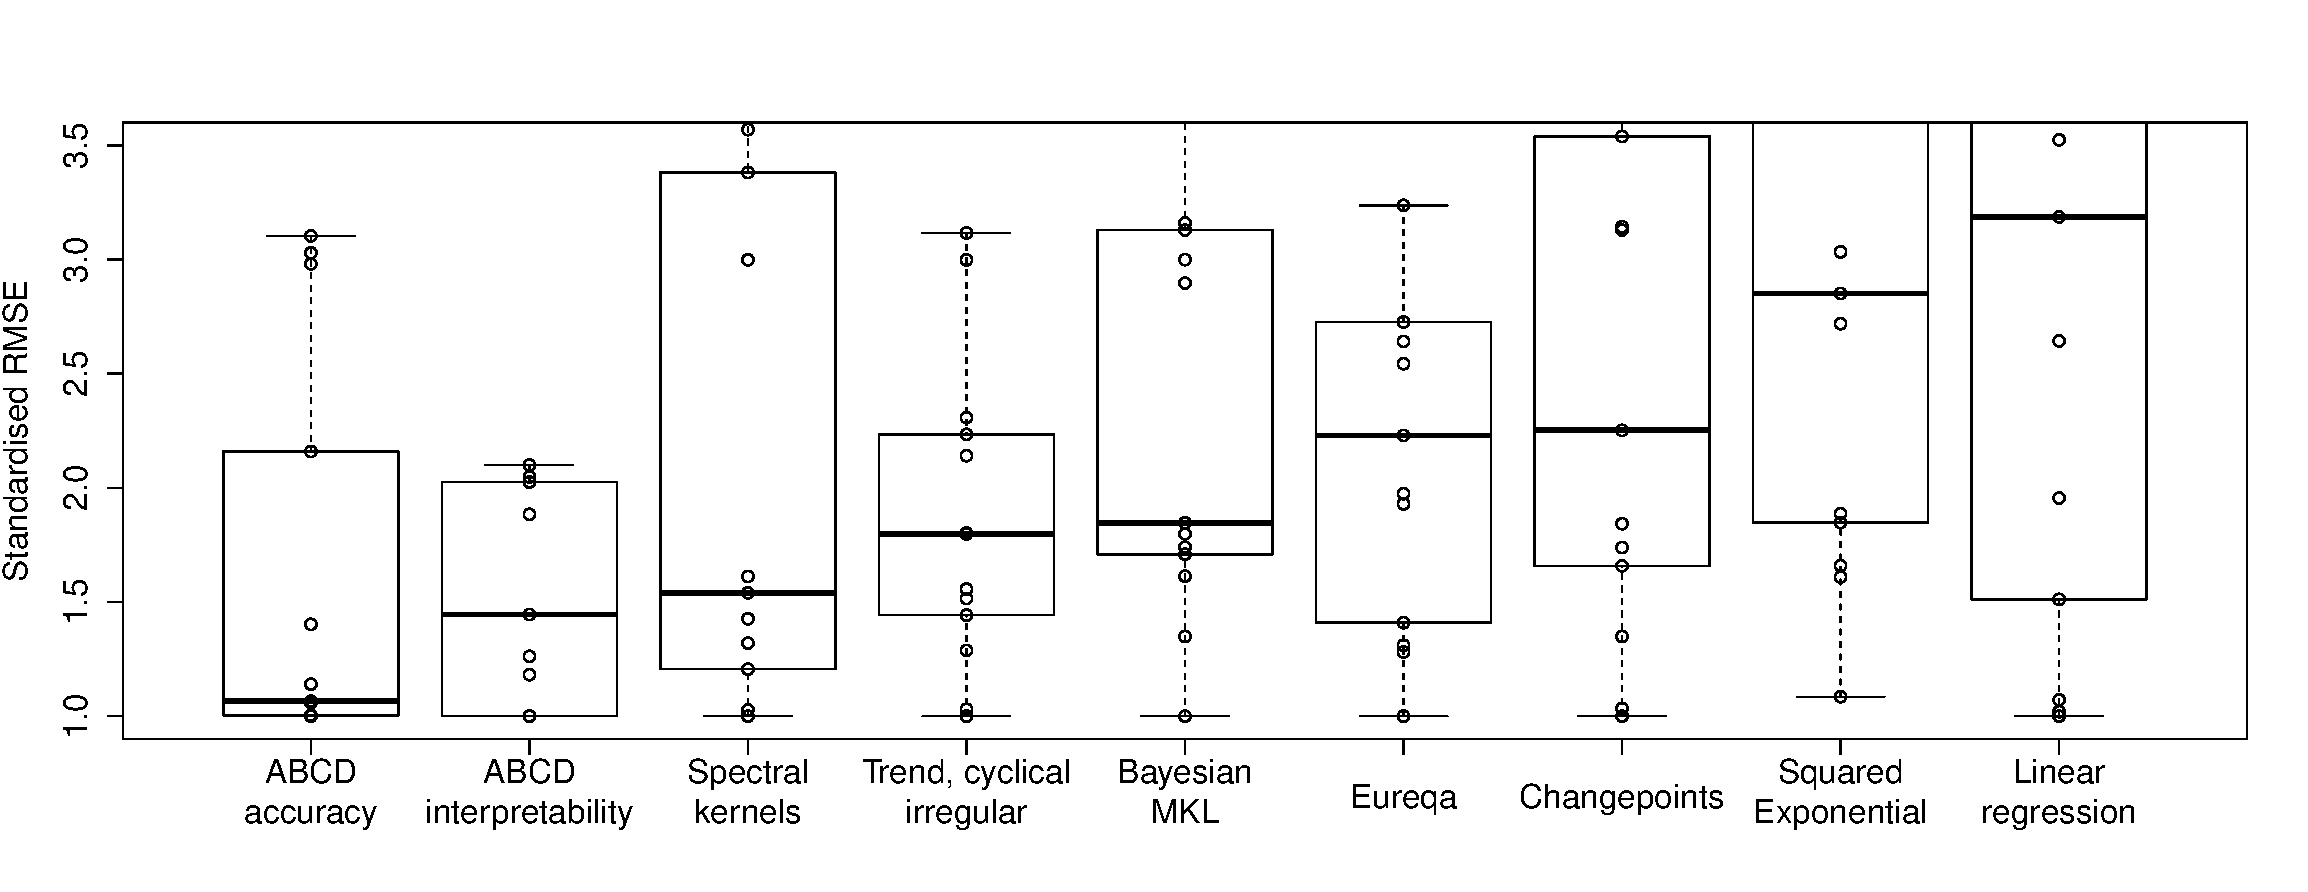
\includegraphics[width=1.02\textwidth]{\grammarfiguresdir/comparison/box_extrap_wide}
\caption[Comparision of extrapolation error of all methods on 13 time-series datasets.]
{Box plot (showing median and quartiles) of standardised extrapolation RMSE (best performance = 1) on 13 time-series.
The methods are ordered by median.
}
\label{fig:box_extrap_dist}
\end{figure}


Figure~\ref{fig:box_extrap_dist} shows the standardised RMSEs across algorithms.
\procedurename{}-accuracy outperforms \procedurename{}-interpretability.
Both algorithms have lower quartiles than all other methods.

Overall, the model construction methods with greater capacity perform better: \procedurename{} outperforms trend-cyclical-irregular, which outperforms Bayesian \MKL{}, which outperforms squared-exponential.
Despite searching over a rich model class, Eureqa performs relatively poorly, since very few datasets are parsimoniously explained by a parametric equation.

Not shown on the plot are large outliers for spectral kernels, Eureqa, squared exponential and linear regression with values of 11, 493, 22 and 29 respectively.
%All of these outliers occurred on a data set with a large discontinuity (see the call centre data in the supplementary material).

\subsubsection{Interpolation}
To test the ability of the methods to interpolate, we randomly divided each data set into equal amounts of training data and testing data.
The results are similar to those for extrapolation, and are included in the appendix.

%\fTBD{Josh: Can you write about the Blessing of abstraction, and doing lots with a small amount of data?  This might become apparent from plotting the extraplolations.}
%\fTBD{RBG: We could make this point as part of the learning curves for extrapolation by marking the points at which each additional aspect of the structure is found.}





\subsection{High-dimensional Prediction}

\procedurename{} can also be applied to multidimensional regression problems, without any modification.
An experimental comparison with other methods can be found in \Cref{sec:additive-experiments}, where it outperforms a wide variety of multidimensional regression methods.



\subsection{Structure Recovery on Synthetic Data}
\label{sec:synthetic}

Because it is difficult to visualize the structures discovered in multiple dimensions, it is hard to tell from predictive accuracy alone if the search procedure is finding all structure present.
To address this question, we tested our method's ability to recover known structure on a set of synthetic datasets.

For several composite kernel expressions, we constructed synthetic data by first sampling 300 points uniformly at random, then sampling function values at those points from a \gp{} prior.
We then added \iid Gaussian noise to the functions, at various signal-to-noise ratios (\SNR{}).


\begin{table}[ht!]
\caption[Kernels recovered on synthetic data]
{
Kernels chosen by our method on synthetic data generated using known kernel structures. $D$ denotes the dimension of the functions being modeled.
\SNR{} indicates the signal-to-noise ratio.
Dashes - indicate no structure was found.
Each kernel implicity has a \kWN{} kernel included.
}
\label{tbl:synthetic}
\begin{center}
{\small
\begin{tabular}{c c | c c c}
True Kernel & $D$ & \SNR{} = 10 & \SNR{} = 1 & \hspace{-1cm} \SNR{} = 0.1 \\
\hline
$\SE + \RQ$        & 1 & $\SE$ & $\SE \times \Per$ & $\SE$ \\
$\Lin \times \Per$ & 1 & $\Lin \times \Per$ & $\Lin \times \Per$ & $\SE$ \\
$\SE_1 + \RQ_2$    & 2 & $\SE_1 + \SE_2$ & $\Lin_1 + \SE_2$ & $\Lin_1$ \\
$\SE_1 + \SE_2 \times \Per_1 + \SE_3$ & 3 & $\SE_1 + \SE_2 \times \Per_1 + \SE_3$ & $\SE_2 \times \Per_1 + \SE_3$ & - \\
$\SE_1 \times \SE_2$ & 4 & $\SE_1 \times \SE_2$ & $\Lin_1 \times \SE_2$ & $\Lin_2$ \\
$\SE_1 \times \SE_2 + \SE_2 \times \SE_3$ & 4 & $\SE_1 \times \SE_2 + \SE_2 \times \SE_3$ & $\SE_1 + \SE_2 \times \SE_3$ & $\SE_1$ \\
\multirow{2}{*}{ $(\SE_1 + \SE_2) \times (\SE_3 + \SE_4)$ } & \multirow{2}{*}{4} & $(\SE_1 + \SE_2) \times$ \dots & $(\SE_1 + \SE_2) \times$ \dots & \multirow{2}{*}{-} \\
 & & $(\SE_3\times\Lin_3\times\Lin_1 + \SE_4)$ & $\SE_3 \times \SE_4$ &
\end{tabular}
}
\end{center}
\end{table}


Table~\ref{tbl:synthetic} shows the results.
%The first column lists the true kernels we used to generate the data.
%Subscripts indicate which dimension each kernel was applied to.
%Subsequent columns show the dimensionality $D$ of the input space, and the kernels chosen by our search for different \SNR{}s.
%Dashes - indicate that no kernel had a higher marginal likelihood than modeling the data as \iid Gaussian noise. % (\ie equivalent to a constant kernel).
%
For the highest \SNR{}, the method finds all relevant structure in all but one case.
The reported additional linear structure is explainable by the fact that functions sampled from \kSE{} kernels with long length scales occasionally have near-linear trends.
As the noise increases, our method generally backs off to simpler structures, rather than over-fitting.

\subsubsection{Source Code}
Source code to perform all experiments is available on at \url{www.github.com/jamesrobertlloyd/gpss-research}. 
All \gp{} parameter optimisation was performed by automated calls to the GPML toolbox, available at \url{www.gaussianprocess.org/gpml/code/}.


\section{Discussion}

Towards the goal of automating statistical modeling, we developed a system which constructs an appropriate model from an open-ended language, and automatically generates plots decomposing the different types of structure present in the model.

We acheived this by introducing a space of composite kernels defined compositionally as sums and products of a small number of base kernels.  
The set of models included in this space includes many standard regression models.
We proposed a search procedure for this space of kernels which parallels the process of scientific discovery.

We found that the learned structures are often capable of accurate extrapolation in complex time-series datasets, and are competitive with widely used kernel classes and kernel combination methods on a variety of prediction tasks.
The learned kernels often yield decompositions of a signal into diverse and interpretable components, enabling model-checking by humans.
We hope that this procedure has the potential to make powerful statistical model-building techniques accessible to non-experts.

In the next chapter, we'll see how the model components found by this procedure can be automatically described in terms of english-language text.


\section{Open Questions}

While we focus on Gaussian process regression, we believe our kernel search method can be extended to other supervised learning frameworks such as classification or ordinal regression, or to other kinds of kernel architectures such as kernel \SVM{}s.
%However, whether or not such modularity and interpretability is present in other model classes is an open question.






\outbpdocument{
\bibliographystyle{plainnat}
\bibliography{references.bib}
}





\iffalse


\paragraph{Solar irradiance Data} 
Finally, we analyzed annual solar irradiation data from 1610 to 2011 \citep{lean1995reconstruction}.
%
\begin{figure}
\newcommand{\wsd}{0.5\columnwidth}  % width solar decomp
\newcommand{\hsd}{4cm}  % height solar decomp
\newcommand{\srd}{\grammarfiguresdir/decomposition/11-Feb-02-solar-s}  % solar decomp results dir
\newcommand{\mbs}{\hspace{-0.3cm}}  % move back
\begin{tabular}{cc}
\mbs 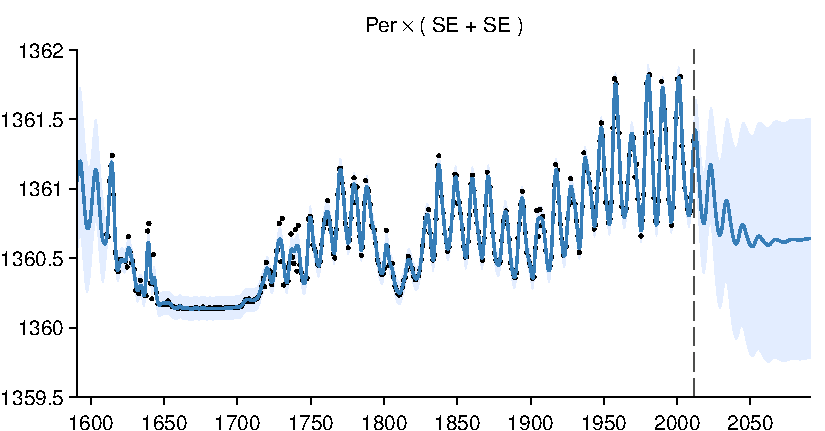
\includegraphics[width=\wsd,height=\hsd]{\srd/02-solar-s_all} &
\mbs 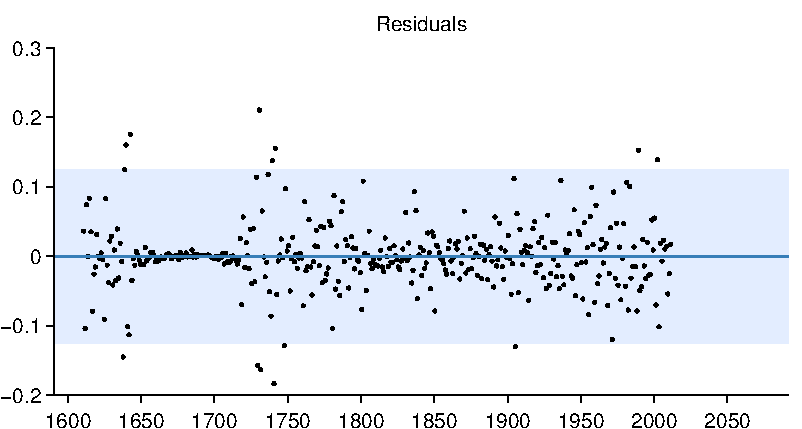
\includegraphics[width=\wsd,height=\hsd]{\srd/02-solar-s_resid}
\end{tabular}
\caption[Decomposition of model discovered on solar irradiance dataset]
{Full posterior and residuals on the solar irradiance dataset.}
\label{fig:solar_decomp}
\end{figure}
%
The posterior and residuals of the learned kernel are shown in figure \ref{fig:solar_decomp}.
%The composite kernel captures the periodic structure in the data, but does not capture the flat structure from 1645 to 1715 during which sunspots were extremely rare.
%but it misses out on another aspect of the data: the flat period from 1645 to 1715 which contains no periodicity and has much smaller variance than the rest of the dataset.
%This corresponds to the Maunder minimum, a period in which sunspots were extremely rare.
%
None of the models in our search space are capable of parsimoniously representing the lack of variation from 1645 to 1715. %, since all of the base kernels apart from \kLin{} are stationary.
%, and it is hard to see how Lin would help in modeling this structure.
%
%
Despite this, our approach fails gracefully: the learned kernel still captures the periodic structure, and the quickly growing posterior variance demonstrates that the model is uncertain about long term structure.
\fi


\iffalse

\subsection{Extrapolation}

\begin{figure}
\centering
\begin{tabular}{c}
\hspace{-0.5cm}
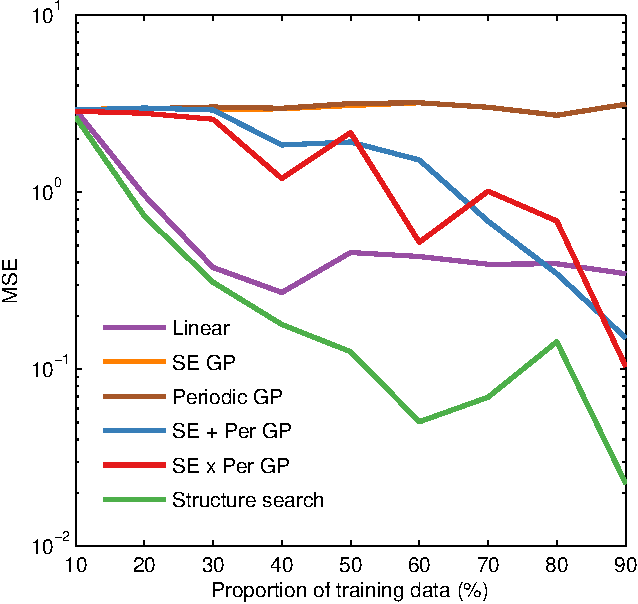
\includegraphics[width=0.5\columnwidth,height=7cm]{\grammarfiguresdir/extrapolation_curves/01-airline-s-ex-curve_hint.pdf}
\end{tabular}
\caption[Comparison of extrapolation performance]
{Extrapolation performance on the airline dataset.  We plot test-set MSE as a function of the fraction of the dataset used for training. 
%\TBD{RBG: Are we using a fixed test set, or the complement of the training set?  It seems like we should do the former, so that the results are less noisy.}
}
\label{fig:extrapolation}
\end{figure}

We compared the extrapolation capabilities of our model against standard baselines\footnotemark.
Dividing the airline dataset into contiguous training and test sets, we computed the predictive mean-squared-error (MSE) of each method.
We varied the size of the training set from the first 10\% to the first 90\% of the data.

Figure \ref{fig:extrapolation} shows the learning curves of linear regression, a variety of fixed kernel family \gp{} models, and our method.  
\gp{} models with only \kSE{} and \kPer{} kernels did not capture the long-term trends, since the best parameter values in terms of \gp{} marginal likelihood only capture short term structure. 
Linear regression approximately captured the long-term trend, but quickly plateaued in predictive performance.
The more richly structured \gp{} models (${\kSE + \kPer}$ and ${\kSE \times \kPer}$) eventually captured more structure and performed better, but the full structures discovered by our search outperformed the other approaches in terms of predictive performance for all data amounts.
%In contrast, a \gp{} with an SE or RQ kernel has unbounded capacity.  However, simply having unbounded capacity does not necessarily translate into the ability to extrapolate, as demonstrate in Figure \ref{fig:extrapolation}.  Only by increasing the amount of structure expressible in a model can we capture the regularities in the data that allow long-range extrapolation.

\footnotetext{
%\NA{
In one dimension, the predictive means of all baseline methods in table \ref{tbl:Regression Mean Squared Error} are identical to that of a \gp{} with an $\kSE{}$ kernel.}
%}



The comparison included three methods with fixed kernel families: Additive \gp{}s, Generalized Additive Models (\GAM{}), and a \gp{} with a standard \kSE{} kernel using Automatic Relevance Determination (\gp{} \kSE{}-\ARD{}).  Also included was the related kernel-search method of Hierarchical Kernel Learning (\HKL{}).
%We compared 5 methods on 5 datasets in terms of mean-squared (MSE) error and predictive likelihood, averaging across 10 data folds.

Results are presented in table \ref{tbl:Regression Mean Squared Error}.
%
% --- Automatically generated by resultsToLatex2.m ---
% Exported at 28-Jan-2013 15:53:45
\begin{table}[h]
\vspace{-0.1cm}
\caption[Comparison of multidimensional regression performance]
{Comparison of multidimensional regression performance.
Bold results are not significantly different from the best-performing method in each experiment, in a paired t-test with a $p$-value of 5\%.
}
\label{tbl:Regression Mean Squared Error}
{\small
\begin{center}
\begin{tabularx}{\textwidth}{l | XXXXX | XXXXX}
 & \multicolumn{5}{c}{Mean Squared Error (\MSE{})} & \multicolumn{5}{c}{Negative Log-Likelihood} \\
 Method & bach & \hspace{-3mm}\parbox{1cm}{concrete} & puma & servo & \hspace{-3mm}\parbox{1cm}{housing}
& bach  & \hspace{-3mm}\parbox{1cm}{concrete} & puma & servo & \hspace{-3mm}\parbox{1cm}{housing}
\\ \hline
Linear reg.
& $1.031$ & $0.404$ & $0.641$ & $0.523$ & $0.289$
& $3.430$ & $1.403$ & $1.881$ & $2.678$ & $1.052$ \\
\GAM
& $1.259$ & $0.149$ & $0.598$ & $0.281$ & $0.161$ 
& $2.708$ & $0.467$ & $1.195$ & $1.800$ & $0.457$ \\
\HKL
& $\mathbf{0.199}$ & $0.147$ & $0.346$ & $0.199$ & $0.151$ 
& - & - & - & - & -\\
\gp{} \acro{\kSE{}-\ARD{}}
& $\mathbf{0.045}$ & $0.157$ & $\mathbf{0.317}$ & $\mathbf{0.126}$ & $\mathbf{0.092}$
& $\mathbf{0.869}$ & $0.398$ & $\mathbf{0.843}$ & $1.429$ & $0.207$ \\
Additive \gp{}
& $\mathbf{0.045}$ & $\mathbf{0.089}$ & $\mathbf{0.316}$ & $\mathbf{0.110}$ & $0.102$
& $\mathbf{0.869}$ & $\mathbf{0.114}$ & $\mathbf{0.841}$ & $1.309$ & $0.194$ \\
\hline
%$\SE{}$ 
%Structure Search & & &&&&&&&&\\
%& $\mathbf{0.044}$ & $0.089$ & $\mathbf{0.315}$ & $\mathbf{0.101}$ & $\mathbf{0.092}$ 
%& $\mathbf{-0.141}$ & $\mathbf{0.054}$ & $\mathbf{0.840}$ & $0.249$ & $\mathbf{0.147}$ \\
%\multirow{2}{1cm}{Search - $\SE{}, \RQ{}$}
%\begin{tabular}{@{}l@{}}Search \\ $\SE{}, \RQ{}$\end{tabular}
$\SE{}, \RQ{}$ Search
& $\mathbf{0.044}$ & $\mathbf{0.087}$ & $\mathbf{0.315}$ & $\mathbf{0.102}$ & $\mathbf{0.082}$
& $\mathbf{0.859}$ & $\mathbf{0.065}$ & $\mathbf{0.840}$ & $1.265$ & $\mathbf{0.059}$ \\
% - All kernels%$\SE{}, \RQ{}, \Lin{}, \Per{}$
%\begin{tabular}{@{}l@{}}Structure Search \\ $\SE{}, \RQ{}, \Lin{}, \Per{}$\end{tabular}
$\SE{}, \RQ{}, \Lin{}, \Per{}$
& $\mathbf{0.509}$ & $\mathbf{0.079}$ & $\mathbf{0.321}$ & $\mathbf{0.094}$ & $\mathbf{0.112}$
& $\mathbf{1.357}$ & $\mathbf{0.114}$ & $\mathbf{0.837}$ & $\mathbf{0.573}$ & $\mathbf{0.151}$ \\
\end{tabularx}
\end{center}
}
\end{table}
% End automatically generated LaTeX
%

\fi


